%Przykładowy plik ułatwiający złożenie projektu dyplomowego inżynierskiego.
%UWAGA: Generowany napis na stronie tytułowej o treści PROJEKT DYPLOMOWY INŻYNIERSKI został zaproponowany przeze mnie i nie jest, póki co, potwierdzony przez władze wydziału. Przed ostatecznym oddaniem tak złożonej pracy należy upewnić się jaka powinna być treść tego napisu. W momencie gdy uzyskam informację na temat treści tego napisu, dokonam niezbędnych zmian w źródłach.

\documentclass[eng,printmode]{mgr}
%opcje klasy dokumentu mgr.cls zostały opisane w dołączonej instrukcji

%poniżej deklaracje użycia pakietów, usunąć to co jest niepotrzebne
\usepackage{polski} %przydatne podczas składania dokumentów w j. polskim
\usepackage{siunitx}
%\usepackage[polish]{babel}%alternatywnie do pakietu polski, wybrać jeden z nich
\usepackage[utf8]{inputenc} %kodowanie znaków, zależne od systemu
\usepackage[T1]{fontenc} %poprawne składanie polskich czcionek

%pakiety do grafiki
\usepackage{graphicx}
\usepackage{subcaption}
\usepackage{psfrag}
\usepackage{caption}

%pakiety dodające dużo dodatkowych poleceń matematycznych
\usepackage{amsmath}
\usepackage{amsfonts}
\usepackage{amsthm}

%pakiety wspomagające i poprawiające składanie tabel
\usepackage{supertabular}
\usepackage{array}
\usepackage{tabularx}
\usepackage{hhline}

%gunwo do kodu
\usepackage{listings}
\lstdefinestyle{java}{
    language=Java,
    basicstyle=\scriptsize,
    aboveskip={1.5\baselineskip},
    columns=fixed,
    showstringspaces=false,
    extendedchars=true,
    breaklines=true,
    tabsize=4,
    prebreak = \raisebox{0ex}[0ex][0ex]{\ensuremath{\hookleftarrow}},
    frame=single,
    showtabs=false,
    showspaces=false,
    showstringspaces=false,
    identifierstyle=\ttfamily,
    keywordstyle=\color[rgb]{0,0,1},
    commentstyle=\color[rgb]{0.133,0.545,0.133},
    stringstyle=\color[rgb]{0.627,0.126,0.941},
    numbers=left,
    numberstyle=\tiny,
    stepnumber=1,
    numbersep=5pt,
    captionpos=b,
    escapeinside={\%*}{*)}
}
\lstdefinestyle{c}{
  belowcaptionskip=1\baselineskip,
  breaklines=true,
  xleftmargin=\parindent,
  language=C,
  showstringspaces=false,
  basicstyle=\footnotesize\ttfamily,
  keywordstyle=\bfseries\color{green!40!black},
  commentstyle=\itshape\color{purple!40!black},
  identifierstyle=\color{blue},
  stringstyle=\color{orange},
  numbers=left,
  stepnumber=1,
  numbersep=5pt,
  inputencoding=latin1
}



\usepackage{hyperref}


%pakiet wypisujący na marginesie etykiety równań i rysunków zdefiniowanych przez \label{}, chcąc wygenerować finalną wersję dokumentu wystarczy usunąć poniższą linię
%\usepackage{showlabels}

%definicje własnych poleceń
\newcommand{\R}{I\!\!R} %symbol liczb rzeczywistych, działa tylko w trybie matematycznym
\newtheorem{theorem}{Twierdzenie}[section] %nowe otoczenie do składania twierdzeń

%dane do złożenia strony tytułowej
\title{Budowa i oprogramowanie robota klasy (2,0) ze zdalnym interfejsem sterowania}
\engtitle{Hardware and software design of remotely controlled (2,0) class robot}
\author{Kornel Mrozek}
\supervisor{Dr inż. Janusz Jakubiak}
%\guardian{dr hab. inż. Imię Nazwisko Prof. PWr, I-6} %nie używać jeśli opiekun jest tą samą osobą co prowadzący pracę

%\date{2008} %standardowo u dołu strony tytułowej umieszczany jest bieżący rok, to polecenie pozwala wstawić dowolny rok

%poniżej jest lista kierunków i specjalności na wydziale elektroniki, należy wybrać właściwe lub dopisać jeśli nie ma odpowiednich
\field{Automatyka i Robotyka (AIR)}
%\specialisation{Robotyka (ARR)}
%\specialisation{Komputerowe sieci sterowania (ARK)}
\specialisation{Systemy informatyczne w automatyce (ASI)}
%\specialisation{Komputerowe systemy zarządzania \\procesami produkcyjnymi (ARS)}
%\field{Elektronika i telekomunikacja (EIT)}
%\specialisation{Akustyka (ETA)}
%\specialisation{Aparatura elektroniczna (EAE)}
%\specialisation{Elektroniczne i komputerowe \\systemy automatyki (ESA)}
%\specialisation{Zastosowania inżynierii komputerowej \\w technice (EZI)}
%\specialisation{Inżynieria dźwięku (EID)}
%\specialisation{Elektronika stosowana \\i optokomunikacja (TEO)}
%\specialisation{Telekomunikacyjne sieci szerokopasmowe (TSS)}
%\specialisation{Teleinformatyczne sieci mobilne (TSM)}
%\specialisation{Sygnały w telekomunikacji cyfrowej (TSC)}
%\specialisation{Teleinformatyczne systemy rozsiewcze (TSR)}
%\field{Informatyka (INF)}
%\specialisation{Systemy informatyki w medycynie \\i technice (IMT)}
%\specialisation{Inżynieria systemów informatycznych (INS)}
%\specialisation{Inżynieria internetowa (INT)}
%\specialisation{Systemy i sieci komputerowe (ISK)}
%\field{Teleinformatyka (TIN)}
%\specialisation{Teleinformatyka (TIN)}

%tutaj zaczyna się właściwa treść dokumentu
\begin{document}
\bibliographystyle{plabbrv} %tylko gdy używamy BibTeXa, ustawia polski styl bibliografii

\maketitle %polecenie generujące stronę tytułową

\tableofcontents %spis treści

%poniżej znajduje się przykładowa treść dalszej części dokumentu, zainteresowanych zachęcam do rozszyfrowania frazy "Lorem ipsum" :)
\chapter{Wprowadzenie}

Robot mobilny klasy 2,0 jest robotem posiadającym dwukołowy napęd różnicowy. Przemieszczania robota umożliwia sterowanie prędkością obrotu koła przymocowanego do danego napędu bez możliwości zmiany kierunku ułożenia koła w  stosunku do platformy robota. 

 \section{Cel projektu}

Celem projektu było zbudowanie fizycznego robota mobilnego 2.0 wraz z napisaniem oprogramowania na mikrokontroler oraz aplikacji, która umożliwia zdalne sterowanie robotem. Komunikacja pomiędzy platformą mobilną a programem sterującym oparta jest na standardzie Bluetooth. Celem pracy było umożliwianie  jak największej interakcji z robotem zarówno w czasie rzeczywistym, jak i za pomocą komend tekstowych, z możliwością pisania skryptów. Główny nacisk położony został na rozwinięcie niezawodnego i rozszerzalnego oprogramowania zarówna na platformie mobilnej, jak i aplikacji desktopowej. 

 \section{Założenie projektowe} 

Projekt zakłada przygotowanie modelu mechanicznego zawierającego dwukołowy napęd różnicowy wraz z  układem elektronicznym umożliwiającym sterowanie silnikiem prądu stałego, jak również odczytem prędkości obrotu wału silnika. W układzie elektronicznym konieczny jest moduł Bluetooth umożliwiający komunikację szeregową z mikrokontrolerem. Oprogramowanie mikrokontrolera osadzonego na robocie zawiera:
\begin{itemize}
  \item komunikację dwukierunkową interfejsu szeregowego
  \item asynchroniczną reakcję na otrzymane wiadomości z zewnątrz
  \item obsługę zliczania impulsów (wymagane przy odczycie prędkości)
  \item układ regulacji prędkości 
  \item zabezpieczenie przed utratą transmisji
\end{itemize}

Aby możliwa była komunikacja między robotem a otoczeniem z zewnątrz wymagane jest przygotowanie protokołu komunikacyjnego dającego aplikacji interfejs na którym może operować. Protokół zawiera wiadomości typu pobierz/zapisz które pozwalają na pobranie z robota wartości i ich nadpisanie. Aplikacja sterująca, zgodnie z celem projektu, ma umożliwiać szeroki zakres form sterowania, opierając się na wyżej wymienionym protokole. Oprogramowanie sterujące zakłada:
\begin{itemize}
  \item możliwość zapisu i odczytu danych w standardzie Bluetooth poprzez wirtualny port COM
  \item możliwość sterowania robotem za pomocą komend tekstowych. Punkt ten zakłada przygotowanie modułu interpretera do wprowadzania komend/skryptów oraz wykorzystanie silnika języka JavaScript
  \item możliwość sterowania w trybie graficznym za pomocą myszki, wizualizacja prędkości oraz konfiguracja robota
\end{itemize}

\chapter{Konstrukcja sprzętowa}

 \section{Platforma mechaniczna}

Platforma mechaniczna robota oparta jest o model Zumo Chassis Kit firmy Pololu. Podstawa mechaniczna zaprojektowana została do konstrukcji robotów o napędzie różnicowym wyposażonym w miniaturowe silniki elektryczne prądu stałego tej samej firmy. Model wyposażony jest w gąsienicowy układ bieżny. Główną zaletą tego rozwiązania jest zwiększenia powierzchni styku z podłożem, co zwiększa przyczepność i zmniejsza prawdopodobieństwo poślizgu poprzecznego. Jest szczególnie istotne w przypadku użycia odometrii przy pomiarze prędkości robota. Platforma skonstruowana została z myślą o używaniu baterii AA, do zasilania robota. Projekt zakładał jednak zastosowanie akumulatora LiPol jako źródła energii. Konstrukcja napędu, jak również rozmiar i cena były przyczyną wykorzystania właśnie tego modelu.

   \begin{figure}[ht]
    \centering
    \begin{subfigure}{.45\textwidth}
     \centering
     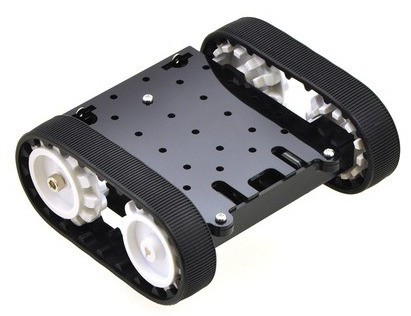
\includegraphics[width=1\textwidth]{images/model_mechaniczny}
  	 \captionof{figure}{Platforma mechaniczna}
     \label{fig:model_mechaniczny}
    \end{subfigure}
    \begin{subfigure}{.45\textwidth}
     \centering
     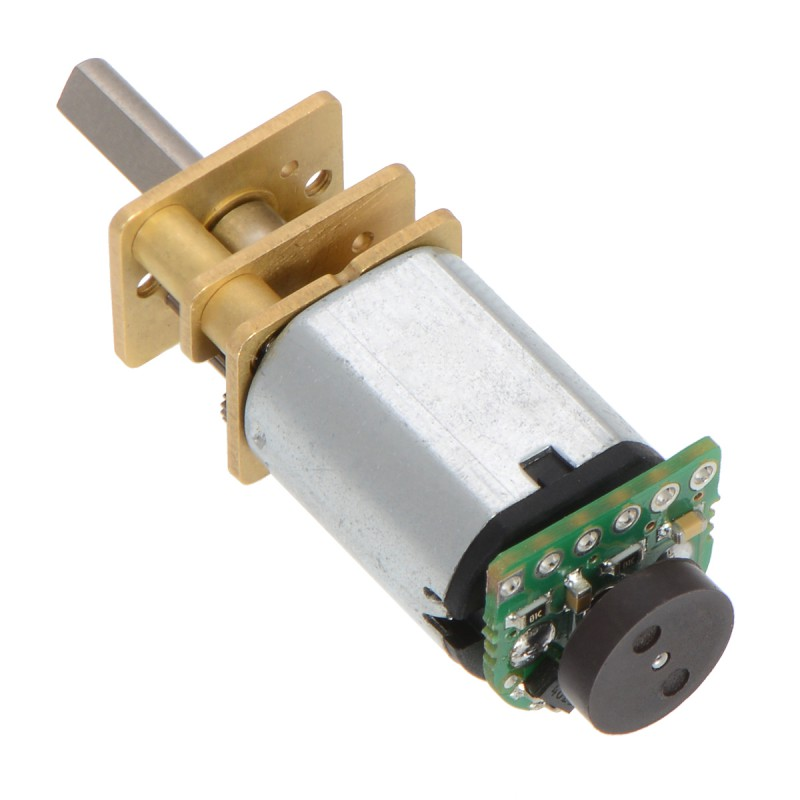
\includegraphics[width=1\textwidth]{images/silnik_enc}
  	 \captionof{figure}{SLinik wrazz enkoderem}
     \label{fig:silnik_enc}
    \end{subfigure}
    \caption{Gotowy moduł nadajnika}
    \label{fig:plytka}
   \end{figure}

Wymiary modelu mechanicznego:
\begin{itemize}
  \item wymiary pełnego modelu: 86[mm] x 98[mm]
  \item odległość pomiędzy kołami (pomiar od środka gąsienicy): 7.5[6mm]
  \item przestrzeń na podstawę elektroniczną:71[mm] x 80[mm]
  \item średnica koła: 1.56[mm]
\end{itemize}

Napędami są miniaturowe silniki Pololu HP z dwustronną osią. Silnik posiada przekładnie 50:1 co ogranicza prędkość obrotową wału silnika zwiększając jednocześnie jego moment. Obustronny wał pozwala na wygodny montaż enkoderów, czyli czujników wykorzystywanych przy pomiarze prędkości obrotowej silnika. Parametry silnika:

\begin{itemize}
  \item Maksymalne napięcie pracy: 9[V]
  \item Prędkość obrotowa dla napięcia 6[V]: 625 obrotów na minutę
  \item Moment obrotowy dla napięcia 6[V]: 1.1 [kg*cm]
  \item Maksymalny prąd dla napięcia 6[V]: 1600[mA]
\end{itemize}

Wybór silnika podyktowany był nie tylko możliwościami jakie oferuje, ale przed wszystkim pełną iteracją z modelem mechanicznym oraz enkoderami (montaż zaprezentowany jest na rysunku powyżej). Dzięki temu konstrukcja była przebiegła szybciej i w dużym stopniu zapobiegła wszelkim błędom montażom. 

 \section{Konstrukcja elektroniczna}
Na konstrukcje elektroniczną robota składają się 4 moduły:
\begin{itemize}
  \item układ Nucleo F401RE z mikrokontrolerem STM32F401
  \item moduł Bluetooth HC-05
  \item zestaw enkoderów magnetycznych 
  \item bazowy obwód łączący układ Nucleo z silnikami 
  \item akumulator LiPol Redox 7.4 V 500mAh
\end{itemize}

  \begin{figure}[ht]
   \centering
   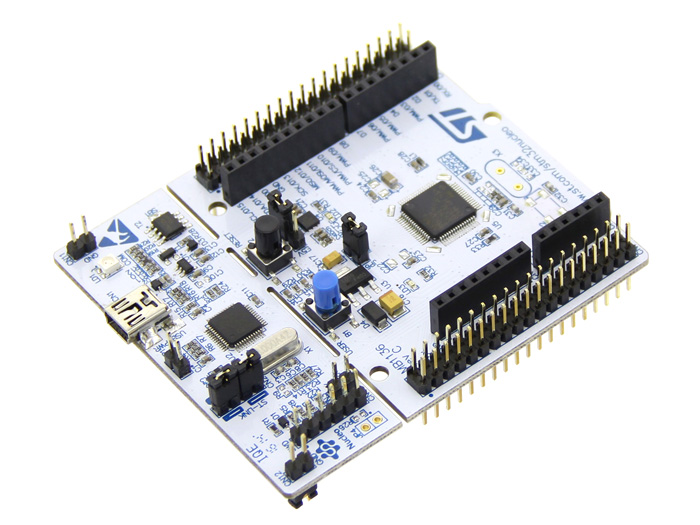
\includegraphics[width=9cm]{images/nucleo}
   \caption{Wizualizacja zasady wyznaczania pozycji}
   \label{fig:nucleo}
  \end{figure} 

Elektronika robota opera się o układ Nucleo F401RE.Sercem układu jest mikrokontroler STM32F401.Posiada on 32-bitową architekturę opartą o rdzeń ARM Cortex M-4 i może być taktowany do 84 MHz. Wydajna jednostka obliczeniowa wraz z sprzętową obsługą operacji na liczbach zmiennoprzecinkowych była kluczowa przy realizacji projektu.  Oprócz szybkiego przetwarzania danych od mikrokontrolera wymagane była sprzętowa realizacja komunikacji szeregowej oraz duża liczba timerów. Obecny mikrokontroler posiada kontroler DMA (ang. Direct Memory Access),pozwalający przeprowadzać transmisję danych bez obciążania procesora, jak również 10 sprzętowych timerów, co pokrywa wymagania projektowanego systemu.
Parametry STM32F401:
\newline Parametry STM32F401:
\begin{itemize}
  \item Częstotliwość taktowania: 84[MHz]
  \item Pamięć trwała Flash: 512kB
  \item Pamięć Static RAM: 96kB
  \item Ilość programowalnych wejść/wyjść: 81
  \item Interfejsy: 3x I2C, 3x USART, 4x SPI, USB 2.0 Full Speed
\end{itemize}

Nie licząc wypowadzeńpinów mikrokontrolera, istotnymi elementami w Nucleo F401RE są stabilizatorynapięcia na 3.3V i 5V z możliwością zasilania bateryjnego od 9V do 12V oraz progrmator/debuger ST-Link v2 . 
\\Komunikacja bezprzewodowa umożliwia moduł HC-05. Techniczne szczegóły opisane są w rozdziale 3.3. Najważniejsze parametry HC-05:
\begin{itemize}
  \item Napięcie zasilania: 3.3[V]
  \item Zasięg: do 10[m]
  \item Komunikacja: UART
  \item Standard: Bluetooth 2.0 + EDR
\end{itemize}

Odczyt prędkości realizowany jest przez enkodery magnetyczneMagnetic Encoder Pair Kit for Micro Metal Gearmotors formy Pololu. Wybór jest wynikał głównie z wyżej wspomnianej integracji z elementami mechanicznymi robota. Podstawą fizyczną działania magnetycznych enkoderów inkrementacyjnych jest efekt Halla.

   \subsection{Bazowy obwód}
   \begin{figure}[ht]
    \centering
    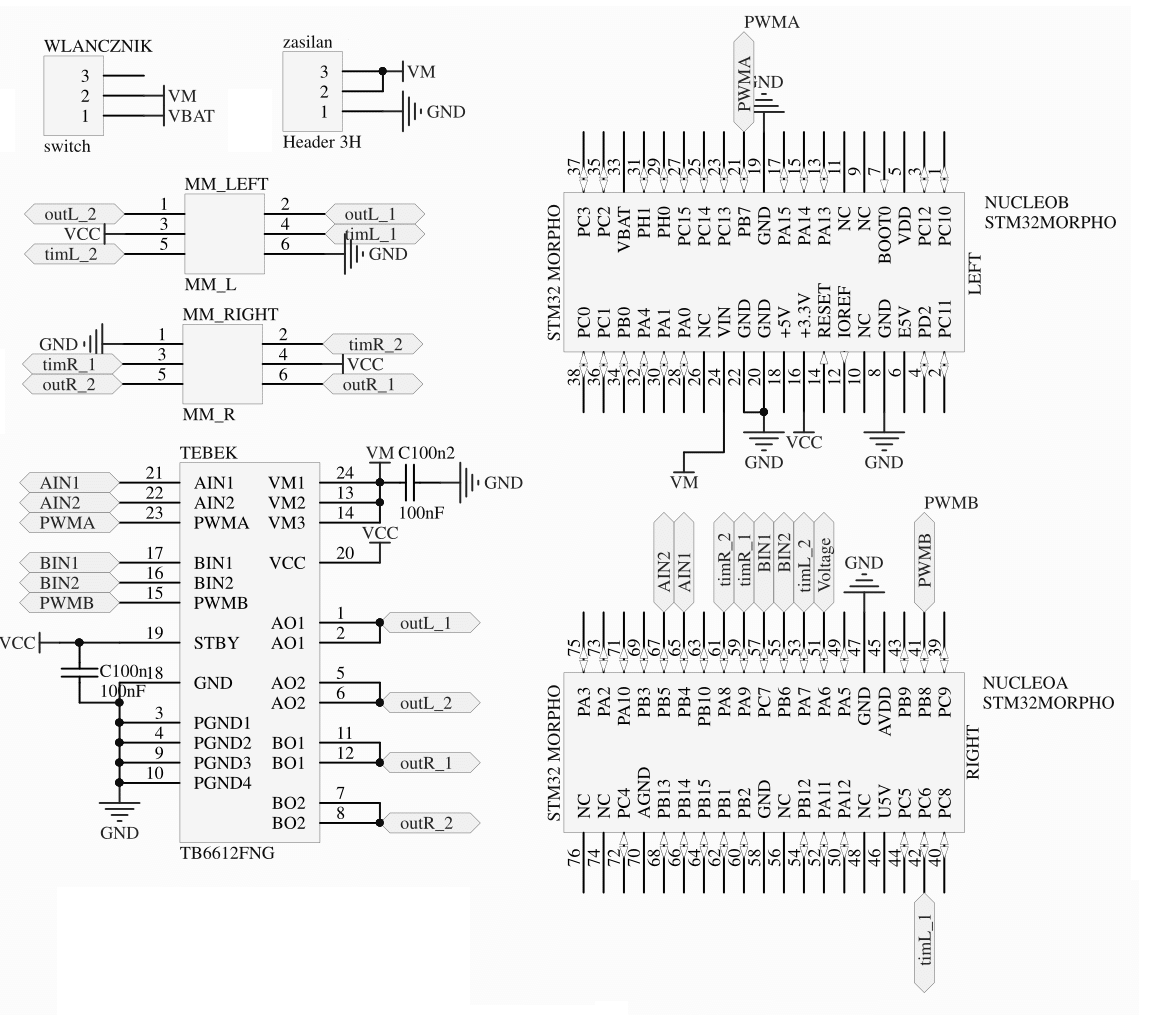
\includegraphics[width=12cm]{images/schemat_elekt}
    \caption{Schemat układu elektronicznego}
    \label{fig:schemat_elekt}
   \end{figure}

Układ elektroniczny zaprojektowany został w programie CircuitMaker firmy Altium. Zadaniem układu było połączenie modułu Nucleo z wyprowadzeniami enkoderami i umieszczenie sterownika silnika. Powszechnym sposobem kontroli silnika prądu stałego jest zastosowanie mostka H. Układ ten pozwala na sterowanie kierunkiem przepływu prądu przez silnik. Funkcja realizowana jest przez układ scalony TB6612FNG, który pozwala na kontrole kierunku obrotów dwóch silników oraz regulacje ich prędkości sygnałem PWM (ang. Pulse Width Modulation). Sygnał zasilający silniki oraz wyprowadzenia enkoderów połączone z układem jest za pośrednictwem złącza micromatch . Wszystkie sygnały podłączone są do mikrokontrolera przez wyprowadzenia Nucelo.
 
\chapter{Oprogramowanie robota mobilnego}
 \section{Struktura oprogramowania}
   \begin{figure}[ht]
    \centering
    \includegraphics[width=1\textwidth]{images/ogol}
    \caption{Schemat blokowy głównego algorytmu robota}
    \label{fig:ogol}
   \end{figure}

Oprogramowanie napisane jest w języku C korzystając z bibliotek HAL (Hardware Abstraction Layer) udostępnionych przez firmę STMicroelectronics. Powyższy schemat pokazuje rozwiązanie podstawowej funkcjonalności robota, czyli regulacji prędkości. Stan robota wyrażonych jest zmiennych globalnych, które poszczególne procedury modyfikują wartość. Cienkie strzałki wskazują kierunek przepływu danych, natomiast grube wskazują na przerwania sprzętowa wyzwalające dane funkcję obsługi. Bezpośrednia zmiana wypełnienia sygnału PWM oraz kierunek obrotu silników za pomocą wiadomości została zaznaczona linią przerywaną. Modyfikacja tych wartości nie jest możliwa podczas trybu regulacji prędkości i wymaga wyłączenia tej procedury( Zagadnienie jest omówione w rozdziale piątym). Przedstawione na schemacie procedury opisane są w dalszej części tego rozdziału. 

 \section{Konfiguracja mikrokontrolera}

Konfiguracja mikrokontrolera wykonana jest przy użyciu oprogramowania STMCubeMX. Pozwala one w bezpieczny i wygony sposób dokonać konfiguracji.

   \begin{figure}[ht]
    \centering
    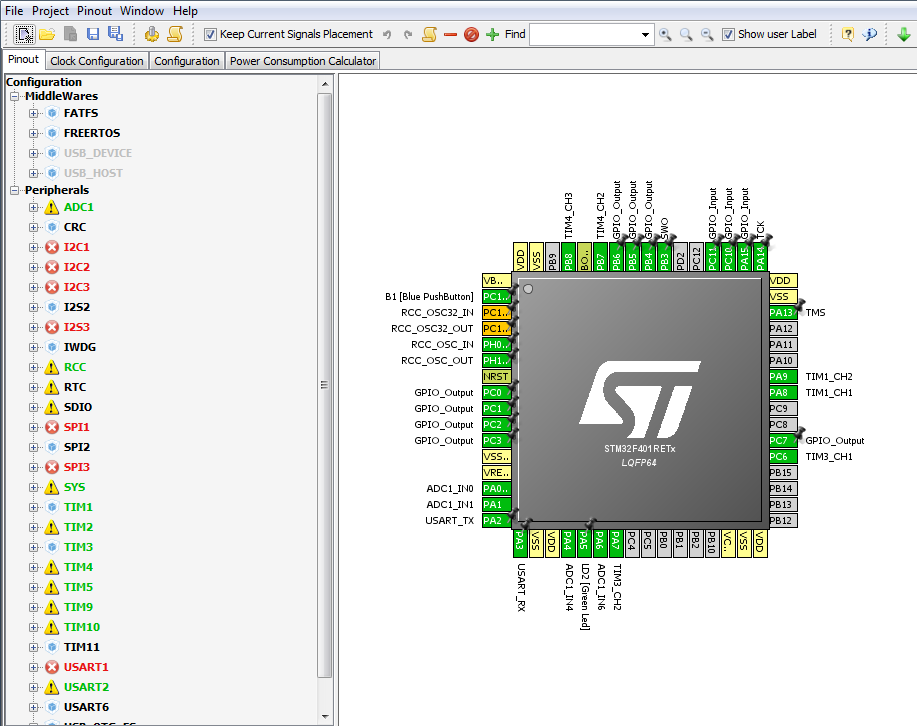
\includegraphics[width=1\textwidth]{images/cubemx1}
    \caption{Konfiguracja pinów mikrokontrolera}
    \label{fig:cubemx1}
   \end{figure}

   \begin{figure}[ht]
    \centering
    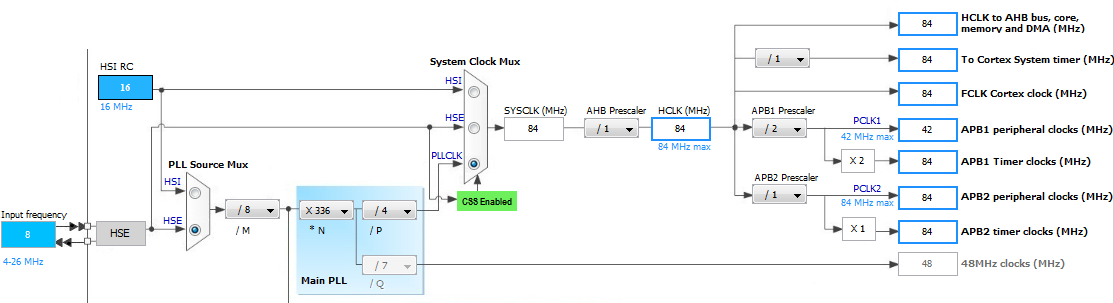
\includegraphics[width=1\textwidth]{images/clock}
    \caption{Konfiguaracja taktowania}
    \label{fig:clock}
   \end{figure}

Mikrokontroler jest taktowany z częstotliwością 84 MHz. Źródłem taktowania jest rezonator kwarcowy 8 MHz, którego częstotliwość jest powielana  przez wewnętrzną pętlę PLL. 

   \begin{figure}[ht]
    \centering
    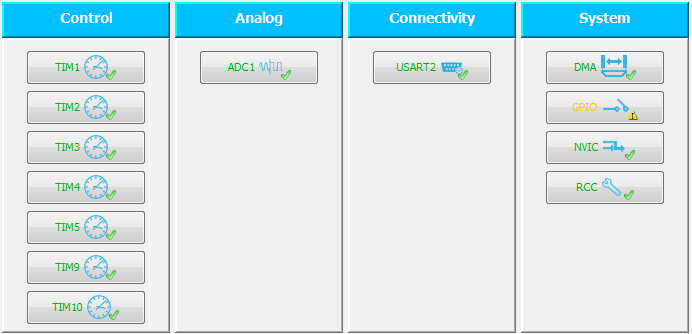
\includegraphics[width=1\textwidth]{images/uC_config}
    \caption{Wykorzystane komponenty STM32F401}
    \label{fig:uC_config}
   \end{figure}

Oprogramowanie wykorzystuje 7 sprzętowych timerów, obsługę transmisji szeregowej UART, magistrale DMA oraz kontroler przerwań NVIC. Oprogramowanie nie zawiera żadnej instrukcji w pętli głównej programu, zachowanie robota jest całkowicie sterowane sprzętowymi przerwaniami. 

 \section{Realizacja komunikacji Bluetooth}

Komunikacja Bluetooth wykorzystuje obsługę dwóch komponentów mikrokontrolera, interfejsu szeregowo UART oraz technika DMA. UART (Universal Asynchronous Receiver and Transmitter) umożliwia asynchroniczne wysyłanie i odbieranie danych przez port szeregowy. Wykorzystanie modułu Bluetooth ogranicza się do połączenia linii danych  TX (wysyłanie) mikrokontrolera z linią danych RX (odbiór) układu HC-06 oraz analogicznie linii RX mikrokontrolera z linią TX modułu. Transmisja bezprzewodowa jest przezroczysta z poziomu mikrokontrolera. Interfejs UART konfigurowany jest przed podanie 4 wartości określających transmisję:
\begin{itemize}
  \item prędkość transmisji (ang. Baud rate)
  \item długość słowa
  \item ilość bitów stopu
  \item bit parzystości (kontrola błędów odbiory danych )
\end{itemize}
Zdecydowałem się na użycie standardowej konfiguracji prędkość: 9600, 8-bitowe słowo, jeden bit stopu, brak bitów parzystości.
\\DMA jest modułem który umożliwia bezpośredni dostęp do pamięci RAM i układów peryferyjnych. Układ DMA umożliwia transfer danych pomiędzy urządzeniem peryferyjnym a pamięcią RAM bez angażowania procesora, którego zadanie ogranicza się do konfiguracji urządzenia. Komponent został użyty do przesyłu i odbioru danych pomiędzy układem UART i dziesięciobajtowym obszarem pamięci RAM. Włączenie odbioru danych szeregowych z użyciem DMA:
\begin{lstlisting}[style=c]
int8_t command[10];
HAL_UART_Receive_DMA(&huart2, command, sizeof(command));
\end{lstlisting}
Argumentami tej funkcji są adres obiektu obsługującego interfejs UART, dziesięciobajtowy obszar pamięci ( tablica dziesięciu bajtów utworzona w globalnej przestrzeni pamięci ) oraz długość tego obszaru. 
\\Asynchroniczność transmisji możliwa jest poprzez obsługę przerwania które generuje UART po zakończeniu transmisji. Biblioteki HAL zapewniają niskopoziomową obsługę przerwań oraz deklaracje zestawu funkcji zwrotnych które zostają wykonane w odpowiedzi na zarejestrowane przerwanie. Obsługa zakończenia transmisji:
\begin{lstlisting}[style=c]
voidHAL_UART_RxCpltCallback(UART_HandleTypeDef *huart)
{
	int8_t response[10];
	int8_t currentCommand[10];
	uint8_t index = 0;
	for(;index < 10; ++index)
		currentCommand[index] = command;
	if(getTimerTimeout(&htim9))
		stopBluetoothTimer();
	commandHandler(currentCommand,response);
	HAL_UART_Transmit_DMA(&huart2,response,10);
	if(getTimerTimeout(&htim9))
		startBluetoothTimer();
}
\end{lstlisting}
Funkcja jest przez bibliotekę HAL wywoływana dla zarejestrowanego przerwania od dowolnego interfejsu UART. Obiekt UART komponentu który wywołał przerwanie jest przekazywany jako argument funkcji. Z uwagi na to, że używany jest jeden interfejs szeregowy nie ma potrzeby sprawdzania czy to on jest źródłem przerwania. Funkcja tworzy tablicę bajtów - response, która wraz z kopią odebranej komendy przekazywana jest do funkcji obsługującej daną wiadomość. Wypełniona odpowiedź wysyłana jest tą samą techniką. Obsługa wiadomości oraz zastosowany timer opisany jest w dalszej części tego rozdziału.
\\Problem, jaki należy rozważyć, w przypadku komunikacji asynchronicznej, jest sytuacja, w której wiadomość jest odbierana zanim wcześniejsza zostanie obsłużona. Dodatkową komplikacja, w tej sytuacji jest użycie DMA, które wypełnia wartości w pamięci z pominięcie pracy, a tym samym kontroli procesora. Praca, na tym samym obszarze pamięci, które wypełnia DMA, podczas obsługi, mogłaby skutkować zmianą wartości tablicy podczas odczytu z niej wiadomości. Z tego powodu, pierwszym etapem w obsłudze przerwania, jest utworzenie kopii tablicy commandi praca na duplikacie. To rozwiązanie, zwiększa stabilność przetwarzania wiadomości, ale nie rozwiązuje problemu całkowicie. Nowa wiadomość mogłaby pojawić się podczas tworzenia duplikatu, co znów generuje ten sam problem. Z pomocą przychodzi tutaj sprzętowa obsługa przerwańw mikrokontrolerach STM. Przetworzenie wiadomości wywoływana jest w obsłudze przerwania, które kończy się dopiero po zaaplikowaniu komendy. Kontroler przerwań NVIC, w przypadku takiego samego priorytetu, tworzy kolejkę LIFO przerwań i a następnie kolejno przekazuje sterowanie, po zakończeniu aktualnie wywołanej funkcji obsługi. Z tego powodu handler nie wywoła się przed zakończeniem przetwarzania bieżącej komendy. Poza wyżej wymienionymi zabezpieczeniami omawiany błąd eliminowany jest przez konstrukcję protokołu komunikacyjnego z aplikacją sterującą. Zgodnie z nim, aplikacja nie wysyła, następnej wiadomości bez otrzymania odpowiedzi na poprzednią, w przypadku prawidłowej wymiany danych, rozwiązuje ten problem.

 \section{Proces przetwarzania wiadomosci}

W poprzednim rozdziale zaprezentowana jest obsługa przerwania od zakończenia transmisji szeregowej. Obecna jest funkcja „commandHandler” odpowiedzialna za obsługę wiadomości i uformowanie odpowiedzi. Struktura  funkcji „commandHandler” ( dla czytelności pominąłem fragment funkcji,n gdyż nie wpływa to na zrozumienie jej działania):
\begin{lstlisting}[style=c]
int8_t* commandHandler(int8_t* command,int8_t* response)
{
if(command[0] != ‘B’ || command[4] != ‘M’ || command[9] != ‘E’)
returninvalidMessage(response);
if(command[1] == 1)
{
//set speed
returnsetVelocityResponse(command,response);
}
if(command[1] == 2)
{
//get speed
returngetVelocityResponse(command,response);
}
//(…) pominęta część funkcji
if(command[1] == 14)
{
//set direction pins
returnsetMotorsDirection(command,response);
}
if(command[1] == 15)
{
//get direction pins
returngetMotorsDirection(command,response);
}
returninvalidMessage(response);
}
\end{lstlisting}

Działanie prezentowanej funkcji jest ściśle związane z protokołem komunikacyjnym pomiędzy robotem a aplikacją sterującą. Zagadnienie to jest szczegółowo opisane w rozdziale piątym. Początek funkcji sprawdza czy na odpowiednich pozycjach występują wartości stałe i charakterystyczne dla każdej wiadomości, w przeciwnym wypadku wysyłana jest wiadomość informująca o błędzie. Następnie na podstawie identyfikatora wiadomości wywoływana jest konkretna funkcja obsługująca daną wiadomość, a jeżeli podany identyfikator nie jest znany zwracany jest błąd. 
\\Obsługa wiadomości zaprezentowana będzie na przykładzie komendy ustalające prędkość zadaną  w układzie regulacji:
\begin{lstlisting}[style=c]

int8_t* setVelocityResponse(int8_t* command,int8_t* response)
{
uint8_tindex = 0;
for(;index<10; ++index)
response[index] = 0;
response[0] = ‘B’;
response[1] = command[1];
response[2] = command[2];
response[3] = command[3];
response[4] = command[5];
response[5] = command[6];
if(command[2] == 0&& command[3] == 0&& command[5] == 0&& command[6] == 0)
{
stopMotors();
return response;
}
int8_t data[2];

data[0] = command[2];
data[1] = command[3];
setLeftSpeed = byte2Float(data);

data[0] = command[5];
data[1] = command[6];
setRightSpeed = byte2Float(data);

if(command[7] != 0&& command[8] != 0)
{
data[0] = command[7];
data[1] = command[8];
uint32_t timer = byte2int(data);

startSpeedTimer(timer);
}

return response;
\end{lstlisting}

Każda funkcja początkowo wypełnia odpowiedź zerami i wartościami stałymi. Dla wiadomości typu „ustaw” odpowiedź powinna być identyczna jak komenda przychodząca. Dzięki temu aplikacja sterująca może mieć pewność, że ustawione zostały podane wartości. Pobór fatycznych wartości ustawionych na robocie odbywa się za pomocą wiadomości typu „pobierz”.  Zaprezentowana wiadomość ustawia 3 pozycje: prędkość lewego koła, prędkość prawego koła (w cm/s ) oraz opcjonalnie czas trwania zadanego ruchu. Wiadomości ustawiające prędkość charakteryzują się jeszcze jedną właściwością. Mając wszystkie pola wartości  wypełnione zerami wywołuje się funkcja zatrzymania silników robota. Jest to jedna z form zabezpieczenia. Warunek ten jest sprawdzany od razu po uformowaniu odpowiedzi. Kolejnym etapem jest konwersja odpowiednich bajtów na liczbę zmiennoprzecinkową i zapis wartości do globalnej zmiennej określającej zadaną prędkość dla danego koła. Ostatnim etapem obsługi wiadomości jest ustawienie czasu trwania długości danego ruchu. Jeżeli pola nie są wypełnione zerami wystartuje timer z przesłanymi danymi ilościami milisekund, i po tym czasie zostaną zatrzymane silniki. W przeciwnym razie zadana prędkość będzie się utrzymywała aż do jej zmiany. Po zakończeniu procedury zwracany jest adres z odpowiedzią.

 \section{Zabezpieczenia robota}

Podstawową funkcją wykorzystywaną we każdej formie zabezpieczeń robota jest stopMotors:
\begin{lstlisting}[style=c]
voidstopMotors(void)
{
	setLeftSpeed = 0.0;
	setRightSpeed = 0.0;

	LeftPWM(0);
	RightPWM(0);
	stopSpeedTimer();
}
\end{lstlisting}
Funkcja wyzerowuje wartość zadaną oraz ustawiony PWM, jak również zatrzymuje timer odpowiedzialny za czas trwania ustawionej prędkości. Robot posiada 3 mechanizmy zabezpieczeń. Pierwszym jest wymienione w poprzednim rozdziale wysłanie wiadomości zadającej prędkość z wartościami równymi zero. Kolejnym mechanizmem jest wysłanie niepoprawnej wiadomości. Funkcja przygotowująca odpowiedź informującą o błędzie również zatrzymuje silniki. Ostatnim zabezpieczeniem jest możliwość ustawienia timera Bluetooth ( widoczny jest we fragmencie kodu w podrozdziale 3.2 ). Timer zaczyna odliczanie po otrzymaniu dowolnej wiadomości i gdy następna wiadomość nie pojawi się przed zakończeniem odliczania, silniki są zatrzymywane. Jest to forma zabezpieczenia przed utratą łączności. Domyślnie timer ten jest wyłączony. Włączenie oraz ustalenie czasu odliczania jest możliwe za pomocą wiadomości kontrolnej.

 \section{Realizacja odczytu prędkości}

Aby możliwa była regulacja prędkości wymagane jest sprzężenie zwrotne od faktycznej prędkości osiągniętej przez robota. W tym celu kluczowe jest niezawodne przetwarzanie informacji uzyskanych za pomocą enkoderów. Enkodery zamontowane na wale silników podłączone są to pinów skonfigurowanych jako wejścia kanałów timerów obsługujących ten czujniki. Mikrokontroler STM umożliwia skonfigurowanie timera do trybu Encoder Mode, który wiąże wejście sygnału taktującego licznika z impulsem generowanym przez enkoder. Tryb ten również pozwala na sprzętową analizę kolejności generowanych impulsów wyjściowych, co w wygody sposób pozwala na detekcje kierunku obrotu koła.  (…). Do obliczania prędkości użyty został jeszcze jeden niezależny timer, który o ustawiony interwał aktualizuje globalne zmienne zawierające aktualne prędkości kół robota. 
\begin{lstlisting}[style=c]
voidHAL_TIM_PeriodElapsedCallback(TIM_HandleTypeDef *htim)
{
	if(htim == &htim2)
	{
		leftVelocity = LeftVelocity();
		rightVelocity = RightVelocity();
		htim2.Instance->CNT = encoderTimer - 1;
		HAL_TIM_Base_Start_IT(&htim2);
	}
	//( … )
	else if(htim == &htim3)
	{
		onEncoderOverload(&htim3,&leftTotalTicks);
	}
	Else if(htim == &htim1)
	{
		onEncoderOverload(&htim1,&rightTotalTicks);
	}	
}

\end{lstlisting}
Jest to uniwersalny handler dla wszystkich timerów zarejestrowanych na przerwanie od końca odliczania. Biblioteka HAL obsługuje niskopoziomowo przerwanie timera i wywołuje funkcje obsługi przekazują w argumencie adres obiektu kontrolującego dany licznik. Timer (htim2) odpowiedzialny  za aktualizację prędkości jest obsługiwany na początku zapisuje wyniki funkcji obliczających prędkość oraz zapisuje je zmiennych globalnych. Interwał czasowy dla licznika może być ustalony przez wiadomość kontrolną. Obliczona wartość  jest więc średnią prędkością w ustawionej ramie czasowej.  Z powodu, że interwał aktualizacji prędkości może być ustalany dowolną  szesnastobitową wartością oraz maksymalna prędkość jaką mogą uzyskać koła nie jest stała (zależy od zużycia silników, poziomu naładowania baterii, użytej przekładni i innych czynników ) wymagane było zabezpieczenie przed przekroczeniem maksymalnej wartości timera zanim nastąpi aktualizacja prędkości. Obsługę tej sytuacji zapewnia funkcja:
\begin{lstlisting}[style=c]
void onEncoderOverload(TIM_HandleTypeDef *htim,int32_t *totalTickCounter)
{
if(htim->Instance->CNT >64000&& htim->Instance->CNT <65000)
	*totalTickCounter += (ENCODER_INITIAL + 65000 - htim->Instance->CNT);
else if (htim->Instance->CNT >0&& htim->Instance->CNT <1000)
	*totalTickCounter -= (ENCODER_INITIAL + htim->Instance->CNT);

htim->Instance->CNT = ENCODER_INITIAL;
HAL_TIM_Base_Start_IT(htim);
}

\end{lstlisting}
Argumentami jest adres danego timera oraz adres zmiennej pomocniczej określającej ilość impulsów wysłanych przez enkoder od ostatniej aktualizacji prędkości. Zmienna „totalTickCounter” jest ze znakiem co umożliwia określenie zwrotu prędkości. Prędkość zgodna z przyjętą przednią częścią robota przekracza licznik zmniejszając wartość rejestru przy wartości 0, w związku z czym pod rejestrem, podczas obsługi przerwania,  jest zapisana wartość mniejsza od 65000. Dolne ograniczenie zostało dobrane empirycznie. Analogicznie sytuacja wygląda przy przepełnieniu wartości timera odwrotną prędkością. Zmienna pomocnicza jest inkrementowana lub dekrementowana o obliczoną wartość impulsów.
\\Obliczenie prędkości podczas aktualizacji odbywa się za pomocą funkcji „LeftVelocity” i „RightVelocity”. Obliczanie prędkości koła na przykładzie funkcji „LeftVelocity”:
\begin{lstlisting}[style=c]
floatLeftVelocity(void)
{
leftTotalTicks += (ENCODER_INITIAL -htim3.Instance->CNT);
htim3.Instance->CNT = ENCODER_INITIAL;

float vel = 0.0f;
vel = calcVelocity(leftTotalTicks);
leftTotalTicks = 0;
return vel;
}

\end{lstlisting}

Funkcja dodaje do zmiennej „leftTotalTicks” ilość impulsów wygenerowanych przez enkoder od ostatniej aktualizacji prędkości. Następnie zeruje ilość impulsów, oblicza prędkość liniową w cm/s i zwraca ją. Funkcja obliczająca prędkość liniową:
\begin{lstlisting}[style=c]
floatcalcVelocity(int8_t encoderTicks)
{
float tmp = encoderTicks/TICK_PER_ROUND;
tmp = tmp*2.0*SHORT_PI;
tmp = tmp /(getTimerTimeout(&htim2)*0.0001);
tmp = tmp*RADIUS;
return tmp;
}

\end{lstlisting}

W pierwszym kroku obliczana jest ilość obrotów jakie wykonało koło biorąc po uwagę przekładnie silnika i rozdzielczość samego czujnika . Następnym krokiem jest zamiana ilości obrotów na prędkość kątową wyrażoną w radianach na sekundę. Ostatnim etapem jest uzyskanie prędkości liniowej mnożąc prędkość kątową przez promień koła i zwrócenie wartości.

\\Przedstawione rozwiązanie jest odporne na duże prędkości,  niemniej jednak może się nie sprawdzać w przypadku małych. Korzystając z enkoderów inkrementalnych należy być świadomym niepewności pomiarowych w odczycie ilości impulsów w stałej ramie czasowej, wywołanej brakiem synchronizacji generowanego przez czujniki sygnału i timera wyzwalającego aktualizację. Problem pogłębia fakt, że sama rama czasowa może być ustalona z zewnątrz podczas pracy robota. Bezpieczniejsze byłoby zablokowanie możliwości zmiany ustawień timera, jednakże byłoby to sprzeczne z ideą projektu. Dobrana empirycznie wartość 60 [ms] jest wartością nominalną i zalecaną podczas korzystania z robota, a za zamianę tej wartości przejmuję pełną odpowiedzialność użytkownik. 

\\W stałym interwale czasowym problem pojawia wariancja odczytu impulsów, która rośnie wraz ze zmniejszaniem prędkości. Dla stosunkowo dużych prędkości wariancja odczytanych impulsów jest na tyle niewielka, że można ją pominąć, natomiast przy niewielkich potrafi mocno zaburzyć pomiar. W celu wyznaczenia progu prędkości, dla którego pomiar jest stabilny, przygotowany został eksperyment, którego wynika przedstawiono poniżej. Doświadczenie polegało na 30 krotnym pomiarze prędkości oraz ilości impulsów w ramie czasowej dla ustalonego PWM, który następnie inkrementowany był do nowej wartości. W ten sposób wyeliminowano problem błędów wywołanych samym procesem regulacji. 

\\Pomiar odbył się przy pełnym naładowaniu baterii ( 8.2[V]). Całe doświadczenie było w pełni zautomatyzowane poprzez skrypt JavaScript. W tabeli przedstawione są kolejno: wypełnienie PWM, średnia zliczonych impulsów w ramce  60 ms, ich odchylenie standardowe, procent odcylenia w stosunku do średniej oraz uśredniona prędkość.

\begin{tabular}{ | l | l | l | l | l | }
\hline
	PWM & śr. impulsów & Odchyl. standardowe & Stosunek odch do śr [\%] & Prędkość [cm/s]  \\ \hline
	100 & 6.83 & 0.9 & 13.1412 & 0.7 \\ \hline
	150 & 13.57 & 0.5 & 3.65 & 2.17 \\ \hline
	200 & 19.67 & 0.47 & 2.395 & 3.21 \\ \hline
	250 & 25.3 & 0.86 & 3.407 & 4.26 \\ \hline
	300 & 30.87 & 0.67 & 2.171 & 5.24 \\ \hline
	350 & 36.5 & 0.81 & 2.208 & 6.44 \\ \hline
	400 & 44.33 & 1.08 & 2.425 & 7.82 \\ \hline
	450 & 50.4 & 1.28 & 2.542 & 8.8 \\ \hline
	500 & 56.33 & 1.01 & 1.795 & 9.94 \\ \hline
	550 & 61.93 & 0.57 & 0.927 & 11.07 \\ \hline
	650 & 73.6 & 0.66 & 0.901 & 13.39 \\ \hline
	700 & 80.17 & 0.64 & 0.795 & 14.66 \\ \hline
	800 & 93.6 & 0.5 & 0.534 & 17.15 \\ \hline
	900 & 107.23 & 0.45 & 0.42 & 19.63 \\ \hline
	1000 & 120.93 & 0.47 & 0.389 & 22.12 \\ \hline
\end{tabular}
Na podstawie widzimy, że odczyt przy prędkości 0,7 cm/s odczyt jest w bardzo dużym stopniu niestabilny o czym świadczą trzynastoprocentowe wahanie w zliczaniu impulsów. Kolejne odczyty odchylenie od średniej, jednakże błąd na poziome 2.5% wciąż może wprowadzić spore oscylacje przy regulacji prędkości. Błąd poniżej 1% uznany został za miarodajny i na podstawie wyników eksperymentu stwierdzona, że pomiar prędkość powyżej 10 cm/s jest stabilny.



 \section{Układ regulacji}

\chapter{Oprogramowanie aplikacji sterującej}

 \section{Struktura oprogramowania}
 \section{Moduł kontroli komunikacji Bluetooth}
 \section{Moduł sterowania tekstowego}
   \subsection{Użycie silnika JavaScript w aplikacji}
 \section{Moduł sterowania graficznego}
   \subsection{Bazowy blok sterujący}
   \subsection{Bloki sterujące dostępne w aplikacji}
   \subsection{Synchronizacja aktywności bloków}

\chapter{Protokół komunikacyjny}  

 \section{Spis wiadomości kontrolnych}   

  
  \chapter{Prezentacja możliwości wykonanego projektu}

 \section{Dobór nastaw regulator}
 \section{Ustawianie trasy robota za pomocą skrypu}
 \section{Prezentacja graficznego sterowania}

\chapter{Podsumowanie}
\addcontentsline{toc}{chapter}{Bibliografia} %utworzenie w spisie treści pozycji Bibliografia
\bibliography{bibliografia} % wstawia bibliografię korzystając z pliku bibliografia.bib - dotyczy BibTeXa, jeżeli nie korzystamy z BibTeXa należy użyć otoczenia thebibliography

%opcjonalnie może się tu pojawić spis rysunków i tabel
% \listoffigures
% \listoftables
\end{document}


